\section{Wohlstand}
\subsection{Die volkswirtschaftliche Diskussion}
Dies sind die wirtschaftlichen Ziele eines Landes:
\begin{itemize}
	\item Hoher Wohlstand
	\item Tiefe Arbeitslosigkeit
	\item Stabile Preise und Wechselkurse
	\item Nachhaltige Staatsfinanzierung
	\item Stabiles Finanzsystem
\end{itemize}
Der Weg dazu führt entweder über Markt oder Staat.
\subsection{Makroökonomisches Grundmodell}
\begin{minipage}{7cm}
Das Makroökonomische Gleichgewicht ist erreicht wenn die Kurven $AN$ und $AA_K$ sich bei der Kapazitätsgrenze schneiden. 
\begin{itemize}
	\item Preisniveau gemessen an definiertem Güterkorb
	\item Reales Bruttoinlandprodukt, inflationsbereinigte Wertschöpfung
\end{itemize}
\end{minipage}
\begin{minipage}{12cm}
		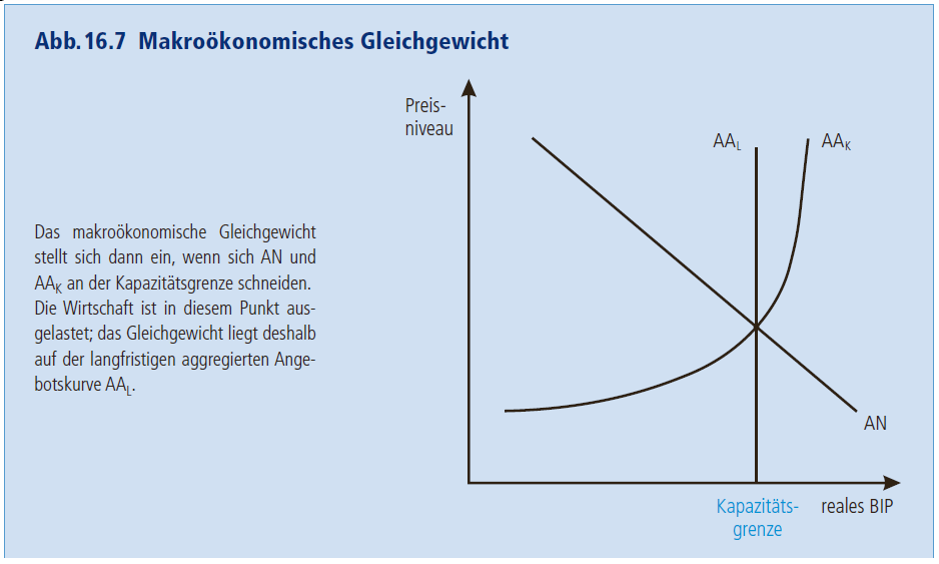
\includegraphics[width=12cm]{images/makro.png}
\end{minipage}


	\subsubsection{aggregierte Nachfrage $AN$}
	Nachfrage nach Gütern (Waren und Dienstleistung) durch die vier volkswirtschaftlichen Akteure.
	\begin{itemize}
		\item Haushalt $\rightarrow$ Konsum
		\item Unternehmen $\rightarrow$ Investitionen
		\item Staat $\rightarrow$ Staatsausgaben
		\item Ausland $\rightarrow$ Nettoexporte = Exporte - Importe
	\end{itemize}
	\subsubsection{langfristig aggregiertes Angebot $AA_L$}
	Beziehung zwischen Produktionsfaktoren. Die Kapazitätsgrenze ist unabhängig vom Preisniveau.
	\begin{itemize}
		\item Arbeit
		\item Kapital
		\item Technologie
		\item Boden und Ressourcen
	\end{itemize}
	\subsubsection{kurzfristig aggregiertes Angebot $AA_K$}
	An der Kapazitätsgrenze sind die Produktionsfaktoren optimal, aber nicht maximal ausgelastet. Durch Überstunden und maximale Auslastung der Infrastruktur kann die $AA_K$-Kurve über der Kapazitätsgrenze liegen.
\clearpage
\pagebreak
\subsection{Bruttoinlandprodukt (BIP)}
\begin{center}
    Das Bruttoinlandprodult gibt den Gesamtwert aller Güter (Produkte und Dienstleistungen), welche innerhalb eines Jahres innerhalb der Grenzen der Volkswirtschaft hergestellt wurden abzüglich der notwendigen Vorleistungen.
\end{center}
Das Bruttonationaleinkommen wird aufgrund der erbrachten Leistungen des Staatsangehörigen \textbf{unabhängig} der Grenzen errechnet.
\begin{itemize}
	\item Das nominale BIP gibt die Wertschöpfung zu Marktpreisen an.
	\item Das reale BIP gibt die Wertschöpfung inflationsbereinigt an.
	\item Das reale BIP der Schweiz beträgt \textbf{ca. 645 Mia.} Franken.
\end{itemize}
\vspace{0.5cm}
Je höher das Bruttoinlandpordukt desto höher ist die  Lebensqualität und der soziale Fortschritt eines Landes. Hier ist zu erwähnen das bei armen Ländern ein geringes Wachstum zu spürbaren Anstieg der Lebensqualität führt. Um das BIP zu analysieren gibt es drei Ansätze
\begin{itemize}
	\item Produktionsansatz: Wertschöpfung der Wirschaftsakteure
	\item Einkommensansatz: Bezahlung der Produktionsfaktoren
	\item Verwendungsansatz: Wirtschaftssubjekte ihr Einkommen verwenden
\end{itemize}
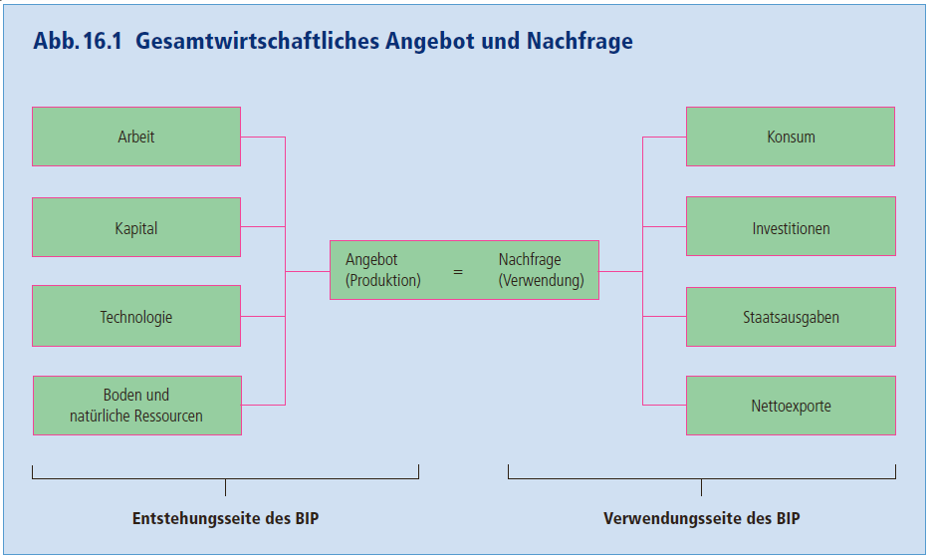
\includegraphics[width=0.8\linewidth]{images/bip.png}
\subsubsection{72er Regel}
\begin{equation*}
	x=\frac{72}{p} \quad \frac{72}{4\%}= 18 Jahre
\end{equation*}

\clearpage
\pagebreak